\section{Interfaces}
All the sensors and actuators are accessed through interfaces, which are the
means by which a system communicates with the outside world.
\begin{center}
    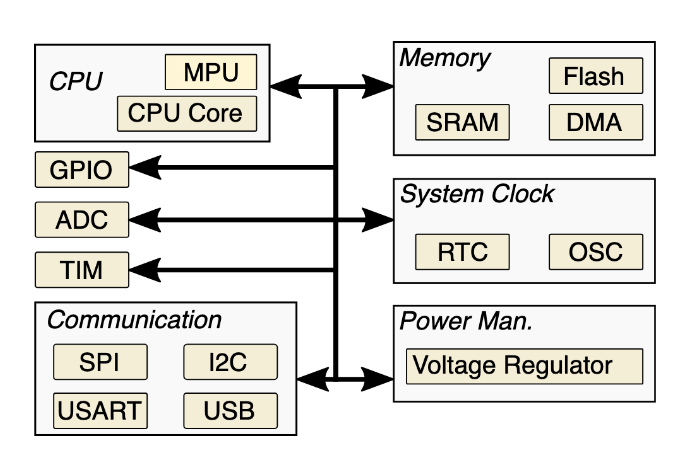
\includegraphics[width=0.6\textwidth]{foto/hardware/cph6/1.png}
\end{center}
Interfaces are hardware block integrated on-chip that:
\begin{itemize}
    \item expose configuration registers to the software;
    \item provide status registers to the software;
    \item provide data registers to the software;
\end{itemize}
They are not just I/O ports but also include \textbf{timers and counters}, \textbf{watchdogs} and \textbf{interrupt controllers}.
A generic peripheral interface is composed of:
\begin{itemize}
    \item \textbf{Control registers}: These registers are used to configure the behavior of the peripheral, such as setting the mode of operation, enabling or disabling certain features, and configuring the timing of the peripheral.
    \item \textbf{Status registers}: These registers provide information about the current state of the peripheral, such as whether it is busy or idle, whether there are any errors, and whether there are any pending interrupts.
    \item \textbf{Data registers}: These registers are used to read and write data to and from the peripheral. For example, in a sensor interface, the data registers would be used to read the sensor data, while in an actuator interface, the data registers would be used to write commands to the actuator.
\end{itemize}
\begin{center}
    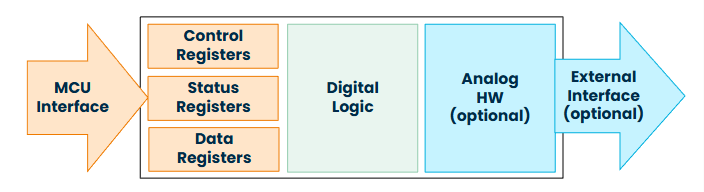
\includegraphics[width=0.6\textwidth]{foto/hardware/cph6/2.png}
\end{center}

To access the registers of a peripheral, the software can use three different
methods:
\begin{itemize}
    \item \textbf{Memory-mapped I/O}: In this method, the registers of the peripheral are mapped to specific memory addresses. The software can read and write to these addresses using standard memory access instructions, just like it would access regular memory.
    \item \textbf{Port-mapped I/O}: In this method, the registers of the peripheral are accessed through specific I/O ports. The software uses special instructions to read and write to these ports, which are separate from regular memory access instructions.
    \item \textbf{Direct register access}: In this method, the software directly accesses the registers of the peripheral using special instructions or by directly manipulating the hardware. This method is typically used in low-level programming or in performance-critical applications where direct access to the hardware is necessary.
\end{itemize}
\subsection{Detecting Peripheral Events?}
To detect peripheral events, the software can use interrupts or polling.
\begin{itemize}
    \item \textbf{Interrupts}: In this method, the peripheral generates an interrupt signal when a specific event occurs, such as when new data is available or when an error occurs. The software can then respond to the interrupt by executing an interrupt service routine (ISR) that handles the event.
    \item \textbf{Polling}: In this method, the software continuously checks the status registers of the peripheral to see if a specific event has occurred. This method can be less efficient than interrupts, as it can consume more CPU resources and may introduce latency in responding to events.
\end{itemize}
\begin{center}
    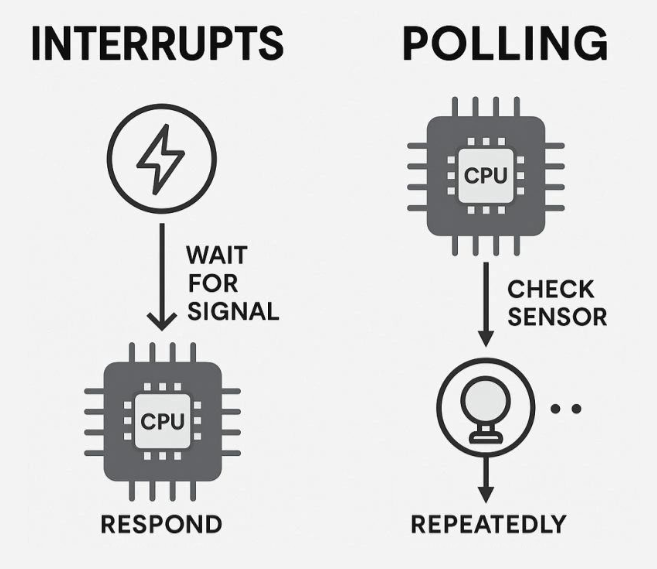
\includegraphics[width=0.6\textwidth]{foto/hardware/cph6/3.png}
\end{center}